\documentclass[11pt,reqno]{amsart}
\usepackage{geometry}                % See geometry.pdf to learn the layout options. There are lots.
\geometry{letterpaper}                   % ... or a4paper or a5paper or ... 
\usepackage[parfill]{parskip}    % Activate to begin paragraphs with an empty line rather than an indent
%\usepackage{algorithm, algorithmic}

\usepackage{algorithm}
\usepackage{algpseudocode}

\usepackage{graphicx}

\usepackage{verbatim}
\usepackage{amssymb}
\usepackage{amsmath}
%\usepackage{epstopdf}
%\DeclareGraphicsRule{.tif}{png}{.png}{`convert #1 `dirname #1`/`basename #1 .tif`.png}

\newcommand{\RR}{I\!\!R} %real numbers
\DeclareMathOperator{\diag}{diag}

\algnewcommand{\Inputs}[1]{%
  \State \textbf{Inputs:}
  \Statex \hspace*{\algorithmicindent}\parbox[t]{.8\linewidth}{\raggedright #1}
}
\algnewcommand{\Initialize}[1]{%
  \State \textbf{Initialize:}
  \Statex \hspace*{\algorithmicindent}\parbox[t]{.8\linewidth}{\raggedright #1}
}

\title[RVD2]{RVD2: An ultra-sensitive variant detection model for heterogeneous population sequencing}
\author{}
%\date{}                                           % Activate to display a given date or no date

\begin{document}
\maketitle

\section{Introduction}

\section{Model structure}\

Given a data matrix $r \in \RR^{J \times N}$ where the element $r_{ji}$ is the count of the reads that contain a non-reference base at position $j$ in experimental replicate $i$. The total count of reads at position $i$ in replicate $i$ is $n_{ji}$. A typical data set is comprised of case and control data sets, $\{ r^{\text{case}} , n^{\text{case}} \}$ and  $\{ r^{\text{control}} , n^{\text{control}} \}$. 

We have developed a hierarchical Bayesian model for this data set because of the nested structure of noise in the data. There is sampling error due to the fact that only a finite number of reads aligned and mapped for each location. There is inter-replicate errors due to experimental protocol and reproducibility. Finally there is sequence context error due to the fidelity of the DNA polymerase enzymes in synthesizing a base. These errors have been shown to depend heavily on the neighboring DNA bases and whether the base is at the end of a molecule or at the center of a molecule.

\subsection{Generative Process} We have codified the statistical structure of these errors in the following generative process (we have used the mean-precision parameterized of the beta distribution): 

\begin{enumerate}
	\item Choose a baseline error rate parameter $\mu_0$ and a inter-location precision parameter $M_0$.
	\item For each location $j$:
	\begin{enumerate}
		\item Sample a location specific error rate parameter $\mu_j \thicksim \text{Beta}(\mu_0, M_0)$
		\item Choose an inter-replicate precision parameter $M_j$
		\item For each replicate $i$:
		\begin{enumerate}
			\item Sample an error rate $\theta_{ji} \thicksim \text{Beta}(\mu_j, M_j)$ for location $j$ in sequencing replicate $i$
			\item Sample the non-reference read count $r_{ji} \thicksim \text{Binomial}(\theta_{ji}, n_{ji})$
		\end{enumerate}
	\end{enumerate}
\end{enumerate}

This model has three levels of sampling. First the baseline error rate across all locations and all replicates is chosen once and for all for the entire data set. Then, based on that baseline error rate, location-specific error rates are sampled. Based on the location specific error rate, replicate-specific error rates are selected. Finally, the observable data, the count of the non-reference reads is sampled.

\begin{figure}[h]
\begin{center}
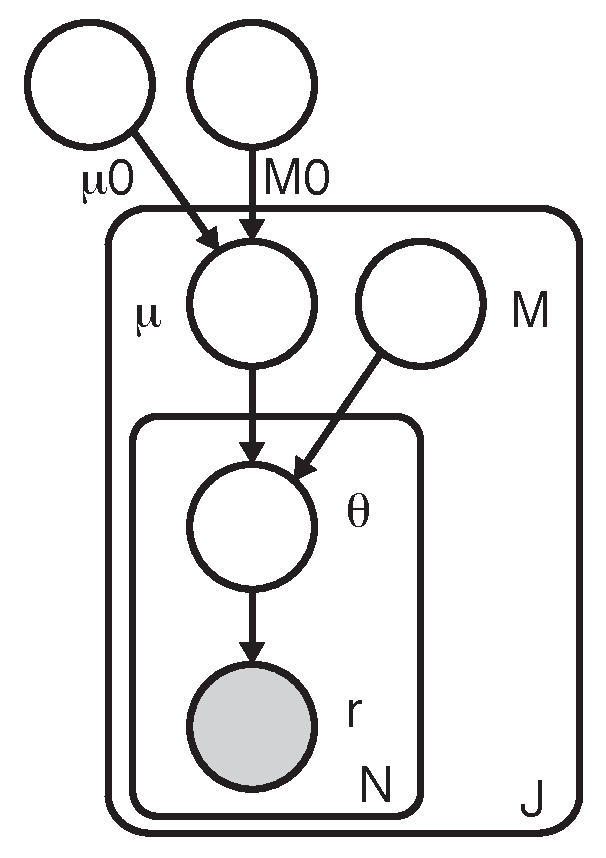
\includegraphics[width=40mm]{pdf_figs/RVD2_model.pdf}
\caption{RVD2 Graphical Model}
\label{fig:graphical_model}
\end{center}
\end{figure}

% Describe graphical model framework here

Given this model structure, the joint distribution over the latent and observed variables for data at location $j$ in replicate $i$ given the parameters is

\begin{equation}\label{eqn:jointpdf}
p \left( r_{ji}, \theta_{ji}, \mu_j | n_{ji}; \mu_0, M_0, M_j \right) = p \left( r_{ji} | \theta_{ji}, n_{ji} \right) p\left( \theta_{ji} | \mu_j; M_j \right) p\left( \mu_j; \mu_0, M_0 \right)
\end{equation}

\begin{gather}
= \frac{ \Gamma(M_0) } { \Gamma(\mu_0 M_0) \Gamma(M_0 (1-\mu_0)) } \mu_j^{M_0\mu_0 -1} (1 - \mu_j)^{M_0 ( 1 - \mu_0) - 1} \\
\cdot \frac{ \Gamma(M_j) } { \Gamma(\mu_j M_j) \Gamma(M_j (1-\mu_j)) } \theta_{ji}^{M_j\mu_j -1} (1 - \theta_{ji})^{M_j ( 1 - \mu_j) - 1} \\
\cdot \frac{ \Gamma(n_{ji}+1) } { \Gamma(r_{ji}+1) \Gamma( n_{ji} - r_{ji} + 1 ) } \theta_{ji}^{r_{ji}} (1 - \theta_{ji})^{n_{ji} - r_{ji}}
\end{gather}

Integrating over the latent variables $\theta_{ji}$ and $\mu_j$ yields the marginal distribution of the data at location $j$ in replicate $i$, 
\begin{equation}
p \left( r_{ji} | n_{ji} ; \mu_0, M_0, M_j \right) = \int_{\mu_j} \int_{\theta_{ji}}  p \left( r_{ji} | \theta_{ji}, n_{ji} \right) p\left( \theta_{ji} | \mu_j; M_j \right) p\left( \mu_j; \mu_0, M_0 \right) d\theta_{ji} d\mu_j
\end{equation}

Finally, assuming the conditional independence structure in the graphical model in Figure~\ref{fig:graphical_model}, the likelihood of the data set is

\begin{equation}
p \left( r ; \mu_0, M_0, M \right) = \prod_{j=1}^J p\left( \mu_j; \mu_0, M_0 \right) \prod_{i=1}^N p \left( r_{ji} | \theta_{ji}, n_{ji} \right) p\left( \theta_{ji} | \mu_j; M_j \right) 
\end{equation}

Instead of attempting to directly compute the posterior distribution, we sample it using a Metropolis-Hastings within Gibbs scheme as described in Section~\ref{sec:algorithm}.

\section{Inference and Hypothesis Testing}

The primary object of inference in this model the joint posterior distribution function over the latent variables,
\begin{equation}
	p(\mu, \theta | r, n; \phi)  = \frac{ p(\mu, \theta, r | n; \phi) } {p ( r | n; \phi)},
\end{equation}
where the parameters are $\phi \triangleq \{\mu_0, M_0, M\}$.

We use a Metropolis-within-Gibbs sampling approach shown in Algorithm~\ref{alg:metro_gibbs} to approximate the posterior distribution. The model parameters are initialized using method-of-moments. Given those parameter estimates we first sample from the marginal posterior distribution for $\mu_j$ given it's Markov blanket using Metropolis Hasting. Then, we sample from the marginal posterior distribution for $\theta_{ji}$ given it's Markov blanket.

\begin{algorithm}[ht]
\caption{Metropolis-within-Gibbs Algorithm}
\label{alg:metro_gibbs}
\begin{algorithmic}[1]

\State Initialize $\theta$, $\mu$, $M$, $\mu_0$, $M_0$
\Repeat
\For {each position j} \Comment{Sample $\mu_j$}
  \State Draw T samples from $p \left( \mu_j |\theta_{ij},\mu_0,M_0\right)$ using M--H
  \State Set $\mu_j$ to the sample median for the T samples
  
  
  \For {each replicate i} \Comment{Sample $\theta_{ji}$}
	\State Sample from $p \left( \theta_{ij} |r_{ij},n_{ij},\mu_j,M \right)$
  \EndFor

\EndFor
\Until {convergence and sample size sufficient}
\end{algorithmic}
\end{algorithm}

Once we have obtained an estimate of the posterior distribution, we test the hypothesis that there is a sub-population of DNA molecules in the pool with a non-reference base at position $j, \forall j \in 1, \ldots, J$. First, we test the hypothesis that the error rate in the case data, $\mu_j^{\text{case}}$ is greater than the error rate in the control data, $\mu_j^{\text{control}}$. If so, then we test the hypothesis that the high error rate is due to excess reads with a particular non-reference base rather than a uniform distribution over all possible non-reference bases.

\subsection{Initialization}

The initial values of the model parameters and latent variables is obtained by a method-of-moments procedure. Essentially, we set the parameter value (population moment) equal to the sample moment. In some cases, the method-of-moments estimate is outside the parameter space. Then, we XXX.

The estimated error probability is calculated from the observed sample
\begin{equation}
 \theta_{ij}=\frac{r_{ij}}{n_{ij}}
\end{equation}

The estimate of parameter $\mu_j$ is obtained using the expected value of $\theta_{ij}$, while $M_j$ is estimated using the moment estimates for the variance of $\theta_{ij}$.
\begin{equation}
 \mu_j=E(\theta_{ij}|\mu_j,M_j)
\end{equation}
\begin{equation}
 M_j=\frac{\mu_j(1-\mu_j)}{Var(\theta_{ij}|\mu_j,M_j)}-1
\end{equation}

Likewise,the estimate of hyperparameters $\mu_o$ and $M_0$ are
\begin{equation}
 \mu_0=E(\mu_j|\mu_0,M_0)
\end{equation}
\begin{equation}
 M_0=\frac{\mu_0(1-\mu_0)}{Var(\mu_j|\mu_0,M_0)}-1
\end{equation}


\subsection{Sampling from $p \left( \theta_{ij} |r_{ij},n_{ij},\mu_j,M \right)$}

We are able to draw samples from $p(\theta_{ji} | r_{ji}, n_{ji}, \mu_j, M_j)$ analytically because of the Bayesian conjugacy between the prior $p(\theta_{ji} | \mu_j, M_j) \thicksim \text{Beta}(\mu_j, M_j)$ and the likelihood $p(r_{ji} | n_{ji}, \theta_{ji}) \thicksim \text{Binomial}(\theta_{ji}, n_{ji})$. 


\subsection{Sampling from $p \left( \mu_j |\theta_{ij},\mu_0,M_0\right)$}

\subsection{Bayesian hypothesis test for high error rate}

To detect a mutation in a specific position, a threshold $\tau$ is set for the posterior difference distribution testing.
\begin{align}
 H_1: \mu_{case}-\mu_{control}\geq\tau \\
 H_2: \mu_{case}-\mu_{control}<\tau
\end{align}

We can calculate the posterior probability of the hypothesis $H_1$ being true by integrating the posterior density over the correct region:

\begin{equation}
 p(H1:\mu_{case}-\mu_{control}\geq\tau)=\int_\tau^\infty p(\mu_{diff} |r,n; \mu_0,M_0)d\mu_{diff}
\end{equation}

We accept the hypothesis $H_1$ if this posterior probability is no lower than 95\%, which means we are 95\% sure that there is a mutation in this position.

ROC curve is plotted to evaluate the performance of the detection algorithm with different threshold for different mutation rate. 


\subsection{$\chi^2$ test for non-uniform base distribution}

We assume that at one position in one experimental replicate, the non-reference reads follows multinomial distribution of $k = 3$ categories, with probability vector $p = (p_1, p_2, p_3)$ where $p_i \geq 0$ for $i =1, 2, 3$ and $\sum_{i=1}^3 p_i = 1$.

The non-reference reads can be because of either mutation or various errors including sampling error, inter-replicated error, $etc$. In theory, the non-reference read counts caused by non-oriented errors should be uniformly distributed among three non-reference categories, namely $p_1=p_2=p_3=1/3$. However, the distribution of non-reference read counts among three non-reference categories caused by mutation theoretically is biased. 

The null hypothesis can be denoted as
\begin{align}
 H_0: p=p_0
\end{align}
where
\begin{align} 
 p_0=(p_1,p_2,p_3), p_1=p_2=p_3=1/3
\end{align}

The null hypothesis is tested using power-divergence family of statistics proposed by Cressie and Read (1984). Considering observed frequencies $\{r_i; i=1,...,k\}$ and expected frequencies $\{E_i; i=1,...,k\}$, by definition the power-divergence family of statistcs indexed by real parameter $\lambda$ is 
\begin{equation}
 2nI^\lambda = \frac{2}{\lambda(\lambda+1)}\sum_{i=1}^k r_i \left[\left(\frac{r_i}{E_i}\right)^\lambda-1\right];\lambda \in R
\end{equation}

Person's $X^2 (\lambda = 1)$ statistics, the log likelih ratio statistics $(\lambda = 0)$, the Freeman-Tukey statistics $(\lambda = -1/2)$ the Neyman modified $X^2 (\lambda = -2)$ are special cases of the family. Cressie and Read (1984) also proposed that when the $\lambda =2/3$, the new power-divergence statistics outcompete the traditional power-divergence statistics. 

Particulaly in our case, Let $(r_1,r_2,r_3)$ denotes the non-reference base frequencies and $\sum_{i=1}^3 r_i = r$. The expected frquencies are $(rp_1, rp_2, rp_3)$. Then the power-divergence statistics can be written as

\begin{equation}
 2nI^\lambda = \frac{2}{\lambda(\lambda+1)}\sum_{i=1}^3 r_i \left[\left(\frac{r_i}{rp_i}\right)^\lambda-1\right];\lambda \in R
\end{equation}

We use $\lambda =2/3$ for the goodness of fit testing.

For each position we have six power-divergence statistics from 6 experimental replicates. We use Fisher's method to combines the six statistics into a single one for inference. Bonferroni correction is applied to maintaining the familywise error rate (FWER). The significance level is chosen as 0.05.

Finally, if read counts in one position passes the Bayesian Hypothesis Testing and fails the Goodness-of-fit Testing, the position will be called.


\subsubsection{Posterior distribution difference sampling}\

Using MCMC sampling, we can obtain the posterior distribution $p \left( \mu |\theta,\mu_0,M_0\right)$ for reference sample and testing sample. In order to compare the difference of position error rate $\mu$ between reference sample and testing sample , a random sampling of posterior distribution is done 

\begin{enumerate}
 \item Randomly  draw one Gibbs sample from $p \left( \mu |r, n, M, \mu_0, M_0\right)$ from reference samples
 \item Randomly draw one Gibbs sample from $p \left( \mu |r, n, M, \mu_0,M_0\right) $ from testing samples
 \item Subtract the former from the later to get one sample for the posterior difference distribution 
\end{enumerate}
Repeat the above three steps until sample size is sufficient.

With the posterior difference distribution of position error rate $\mu$ across replicates obtained, Bayesian inference can be done to summarize the difference. 


\section{Results}
Figure 1 Overall of the process
\subsection{Simulation Results}
\subsection{Comparison Results on Synthetic DNA}
Figure 3 ROC comparison with other methods: varscan/samtools/rvd
\subsection{Empirical Results on Multiple Sclerosis Data}
We tested our method on sequence data from clinical Multiple Sclerosis samples. We expect to see that 

Table: Table of Variants
\subsection{Performance with read depth}
Figure 4 ROC by read depth
picard to thin segment data, showing performance as read depth decreasing


\bibliographystyle{apalike}
\bibliography{bioinfo}
\end{document}  